%	e-Yantra, IIT-Bombay

%	Document Author: Chinmay Patil
%	Date: 11-July,2016
%	Last Edited by: Chinmay
%   Date Last updated: 11-06-2016 

%%%%%%%%%%%%%%%%%%%%%%%%%%%%%%%%%%%%%%%%%%%%%%%%%%%%%%%%%%%%%%%%%%%%%%%%%%%%%


\documentclass[11pt,a4paper]{article}
\usepackage{graphicx}
\usepackage{listings}
\usepackage{graphics}
\usepackage{wrapfig}
\usepackage[T1]{fontenc}
\usepackage[margin=1.2in]{geometry}
\usepackage{tcolorbox}
\usepackage{hyperref}
\usepackage{dingbat}
\usepackage{float}
\usepackage{tocloft}

\begin{document}
\begin{titlepage}
\title{Manual for running wiced sense}
\author{e-Yantra Team}
\date{\today}
\maketitle
\end{titlepage}
\listoffigures
\tableofcontents
    \newpage
	\section{How to use wiced sense GUI ?}
	\subsection{Sensor Data display Page}
	
	 \begin{itemize}
	 \item Open terminal and start lampp local server.
	 
	 	\begin{figure}[h]
    \centering
	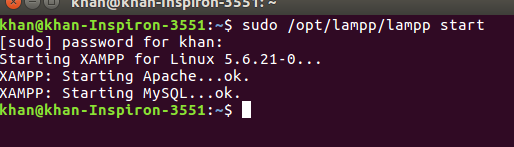
\includegraphics[scale=0.5]{lampstart.png}
	\caption{Starting local server}
	\end{figure}
	 
	 \item Open \href{https://github.com/eYSIP-2016/Wiced-Sense/blob/master/Codes/wiced_web/sensors.html}{sensors.html} page in website.
	 \item Connect XBee using a XBee to usb adapter to a local macSensor.htmlhine.
	 
	 \begin{figure}[h]
        \centering
	    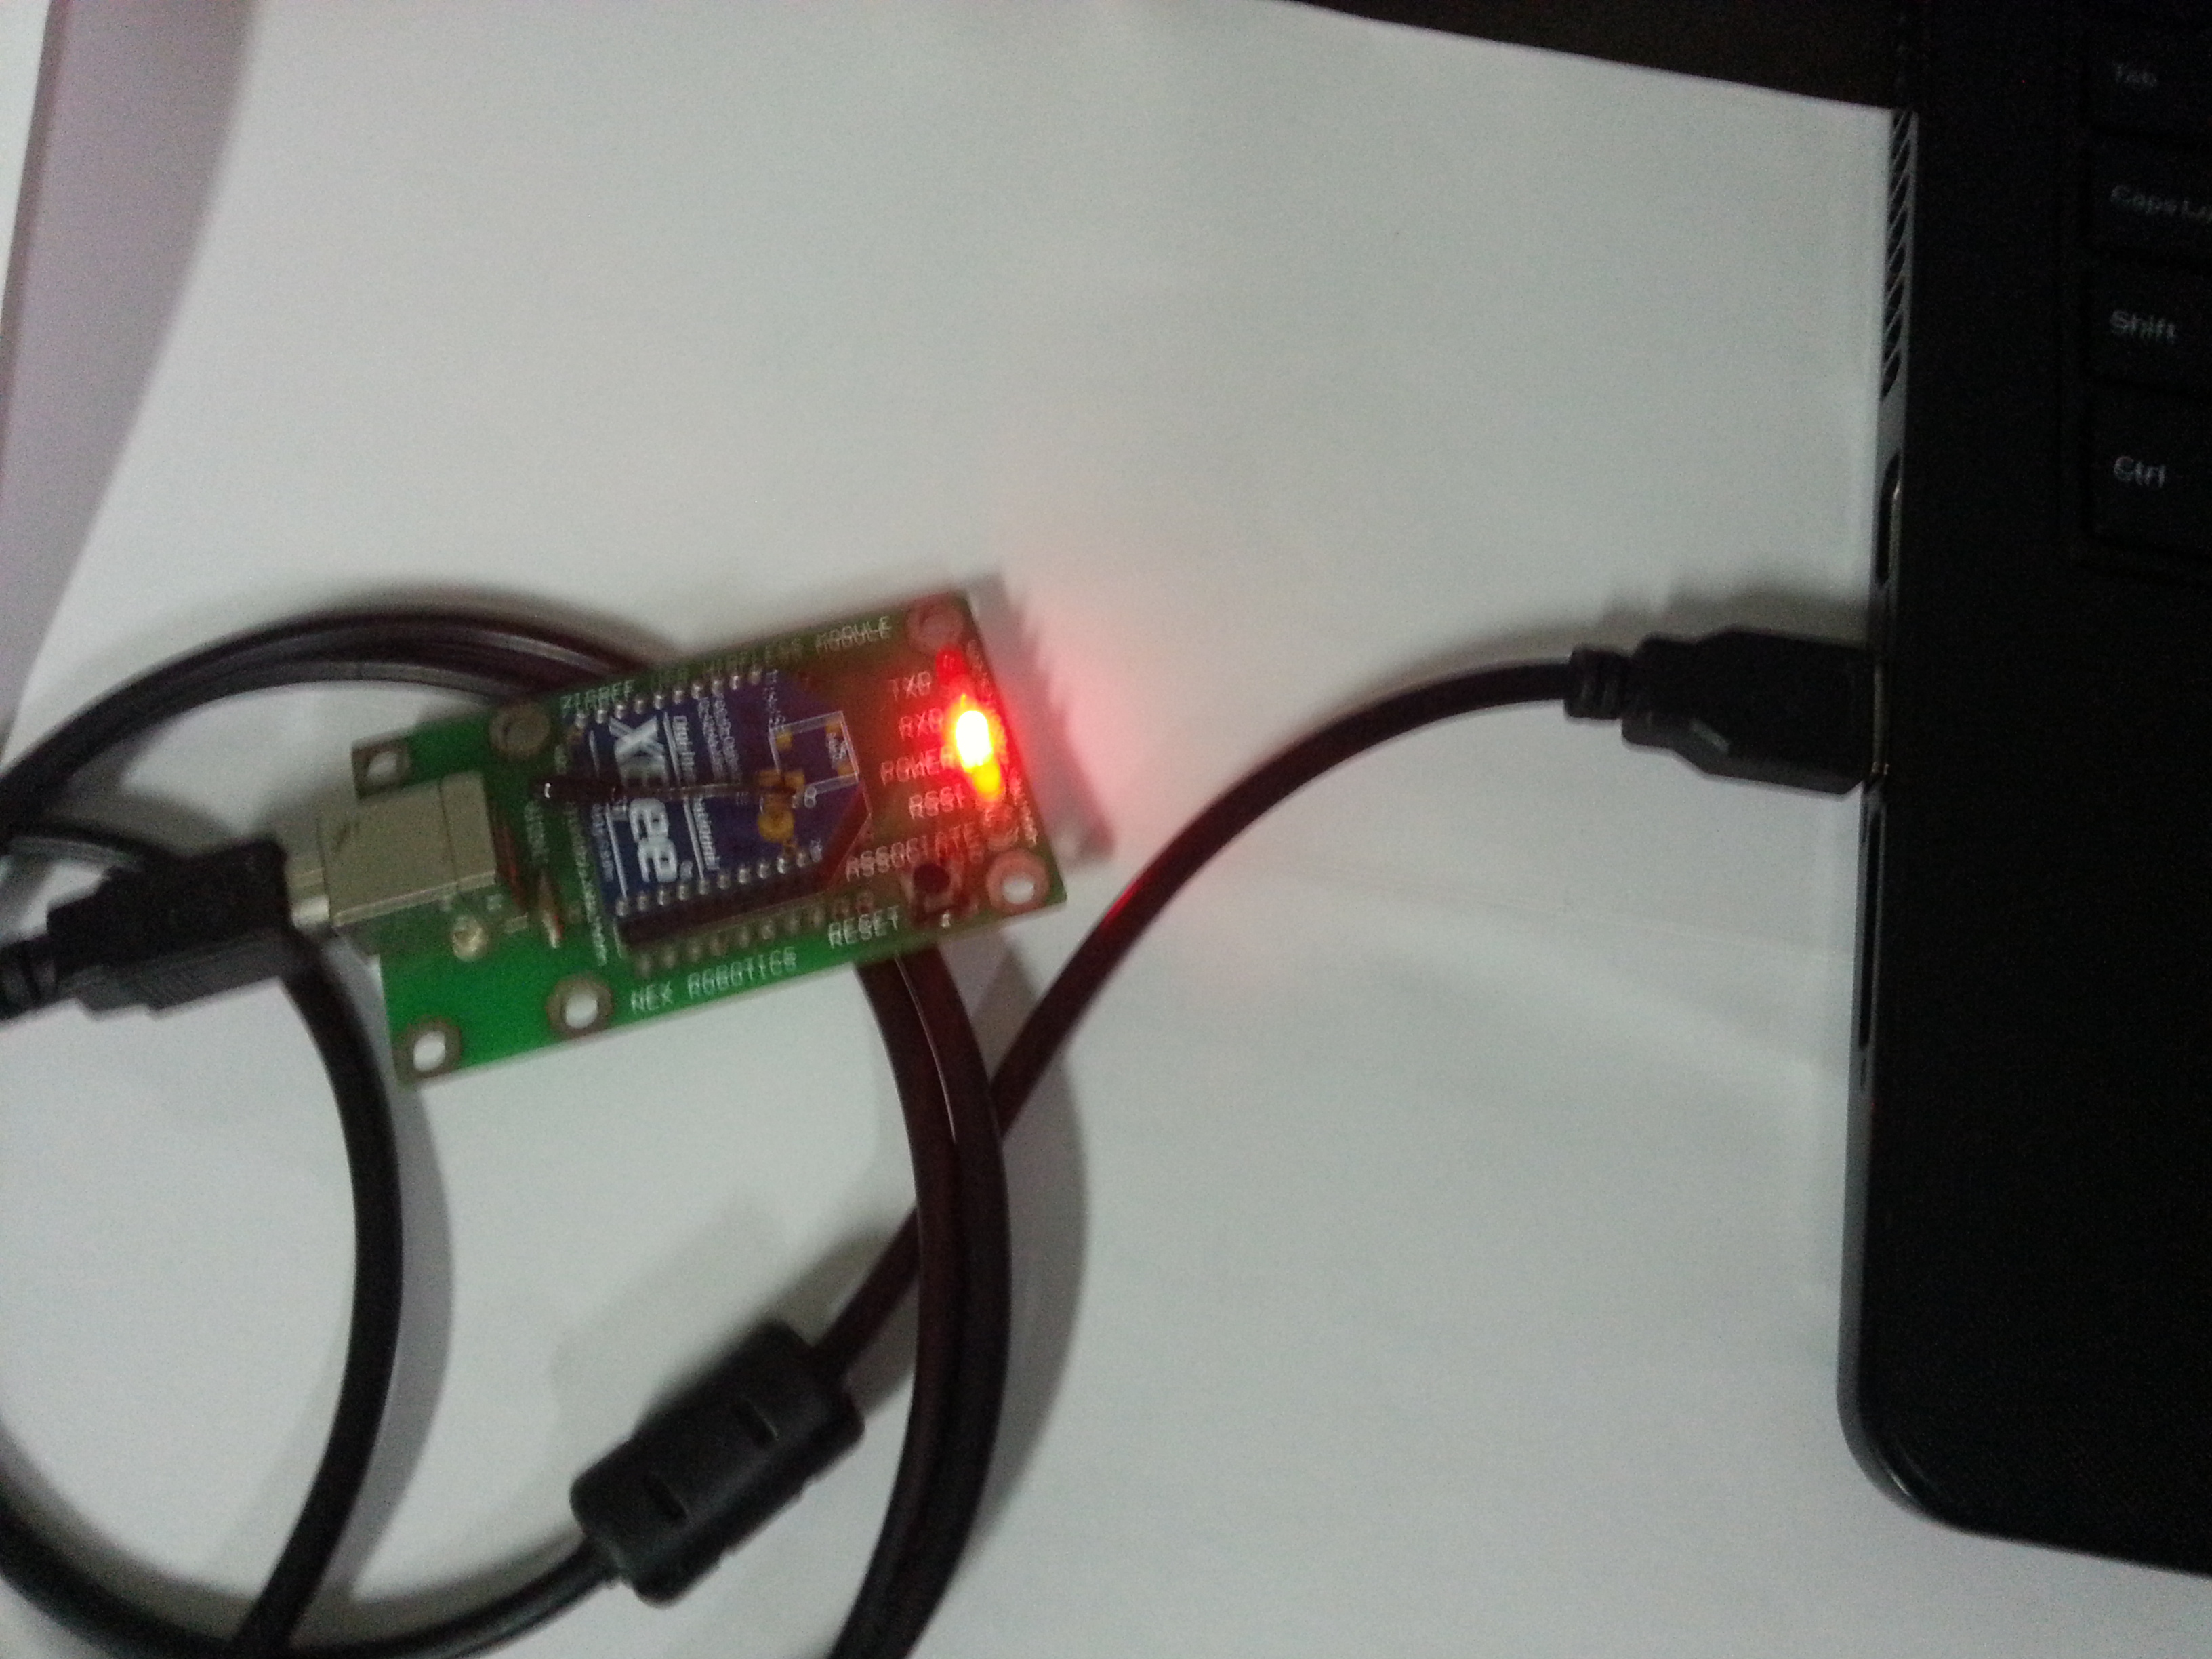
\includegraphics[scale=0.1]{20160722_194935.jpg}
	    \caption{Connecting Xbee to local machine}
	\end{figure}
	 
	 \item Turn ON bluetooth and run wiced.js file in terminal
	 
	 \begin{figure}[h]
    \centering
	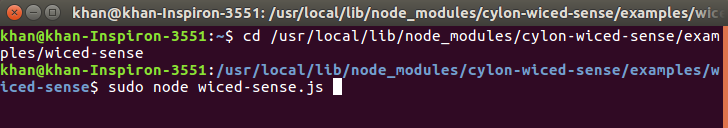
\includegraphics[scale=0.5]{runwicedjs.png}
	 \caption{Running Wiced.js}
	\end{figure}

	 \item As data arrives on terminal the data will be displayed on the page.
	 
	 \newpage 
	 \item Compass and acceleration reading will be displayed immediately according to the sensor data. But data of humidity, temperature, pressure are displayed after some delay of 2-3 sec.
	 
	 \begin{figure}[h]
    \centering{}
    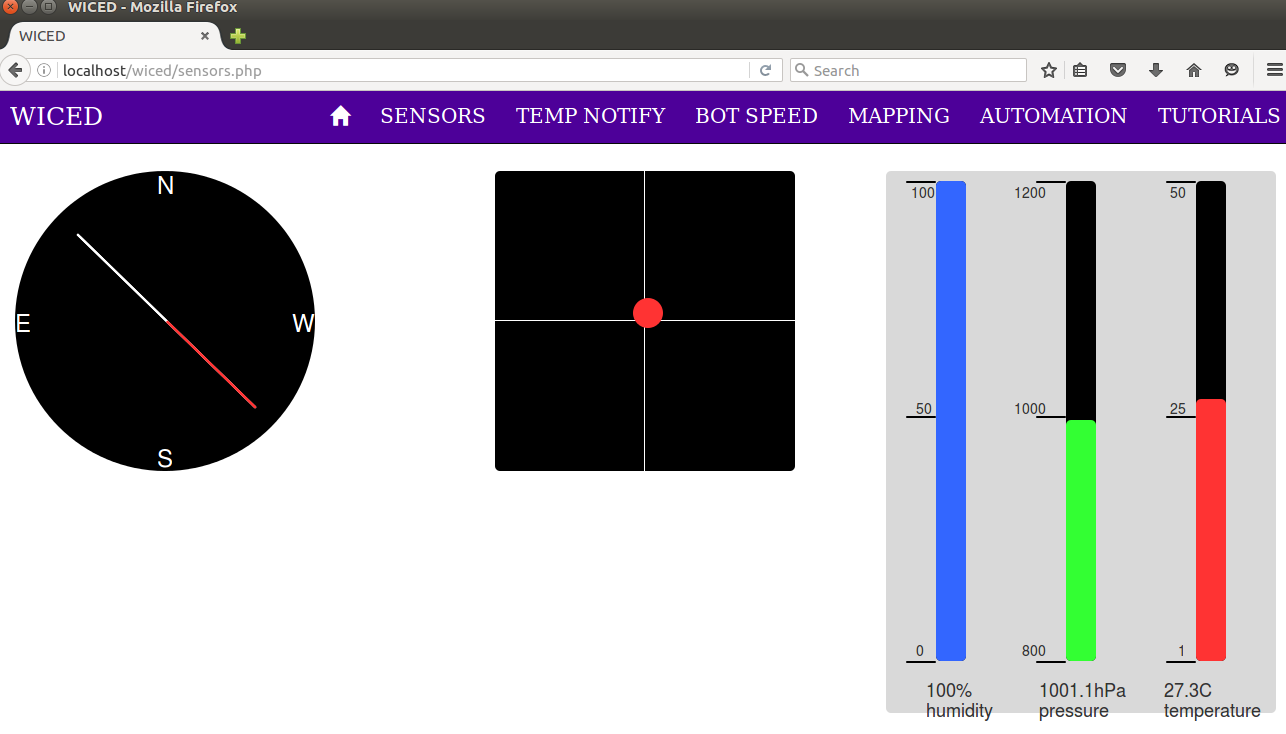
\includegraphics[scale=0.3]{sensor.png}
	\caption{Sensors GUI}
	\end{figure}
	 \end{itemize}
	 
	 
	 
	 \newpage
	 \subsection{How to use temperature notifier ?}
	 
	 \begin{itemize}
	 \item Open terminal and start lampp local server.
	 
	 	\begin{figure}[h]
    \centering
	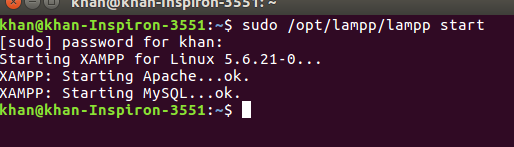
\includegraphics[scale=0.5]{lampstart.png}
		 \caption{Starting local server}
	\end{figure}
	 
	 \item Open \href{https://github.com/eYSIP-2016/Wiced-Sense/blob/master/Codes/wiced_web/temp.html}{temp.html}  page in website.
	 \item Connect XBee using a XBee to usb adapter to a local machine.
	 
	 \begin{figure}[h]
        \centering
	    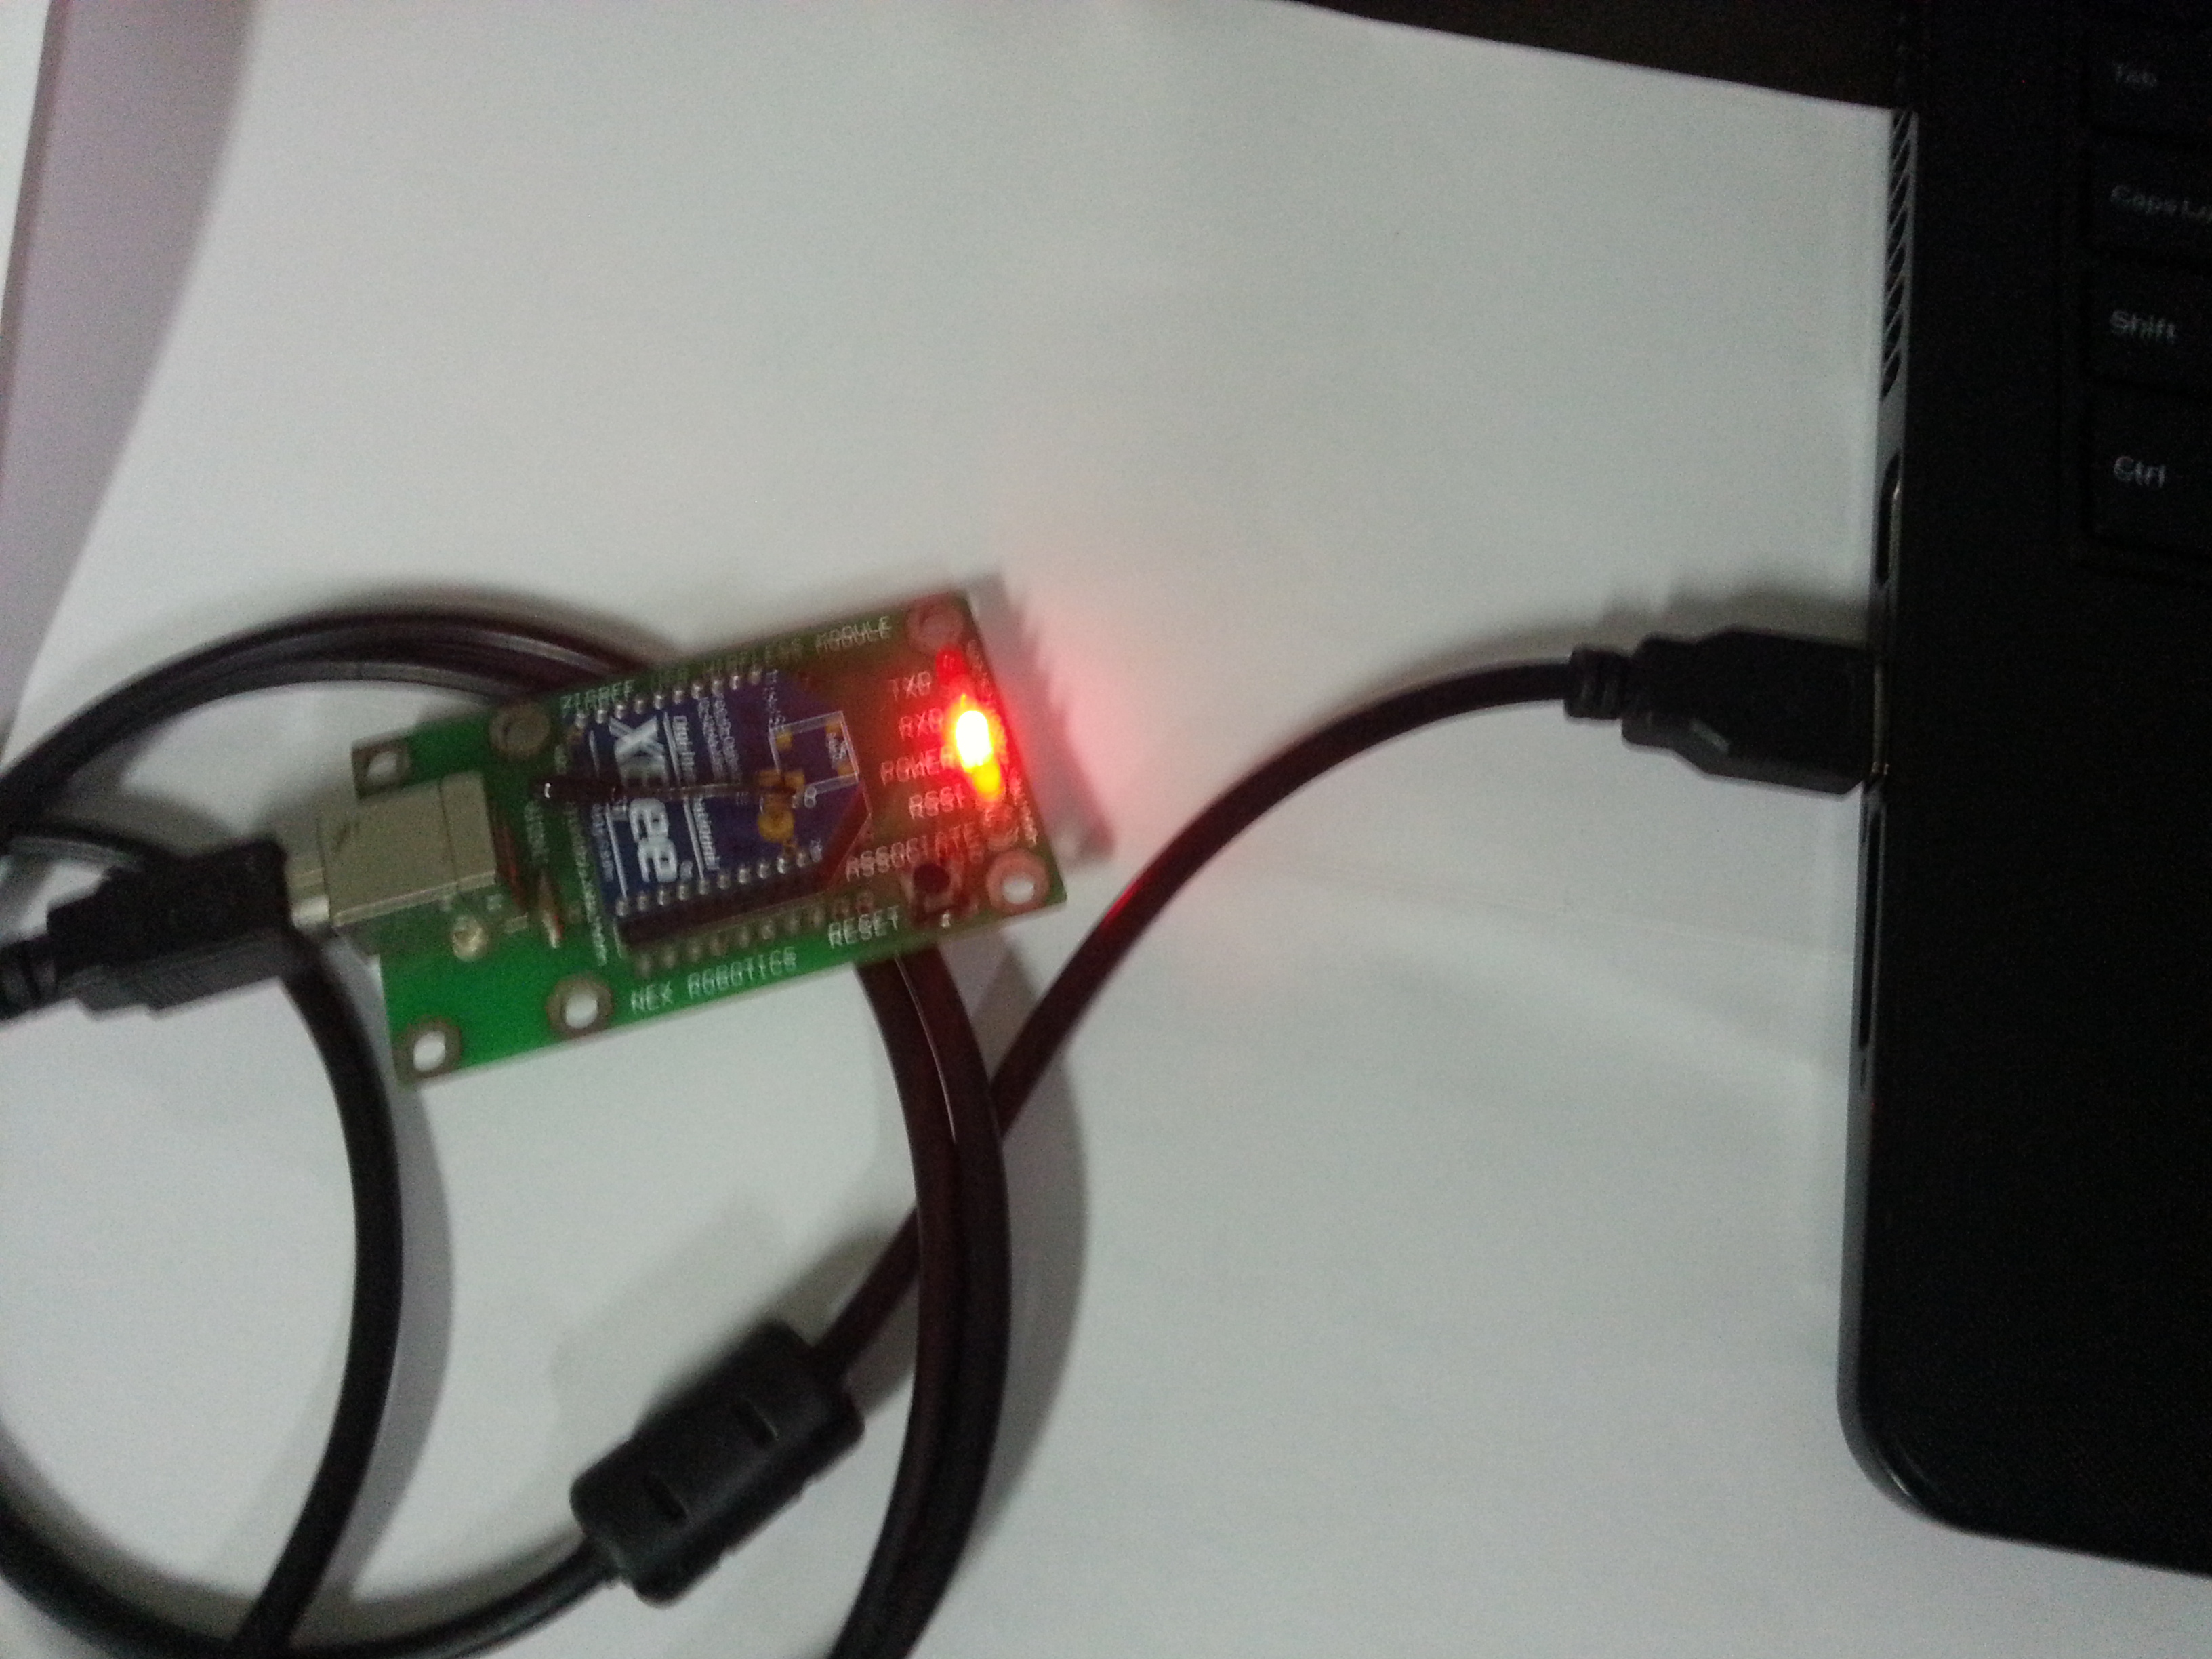
\includegraphics[scale=0.1]{20160722_194935.jpg}
	    	 \caption{Connecting Xbee to local machine}	 
	\end{figure}
	 
	 \item Turn ON bluetooth and run wiced.js file in terminal
	 
	 \begin{figure}[h]
    \centering
	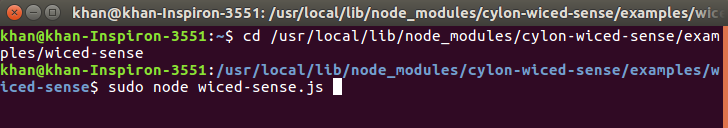
\includegraphics[scale=0.5]{runwicedjs.png}
		 \caption{Running Wiced.js}
	\end{figure}
	 
	 \newpage
	 \item Set temperature of which you need to be notified.
	 \begin{figure}[h]
    \centering
	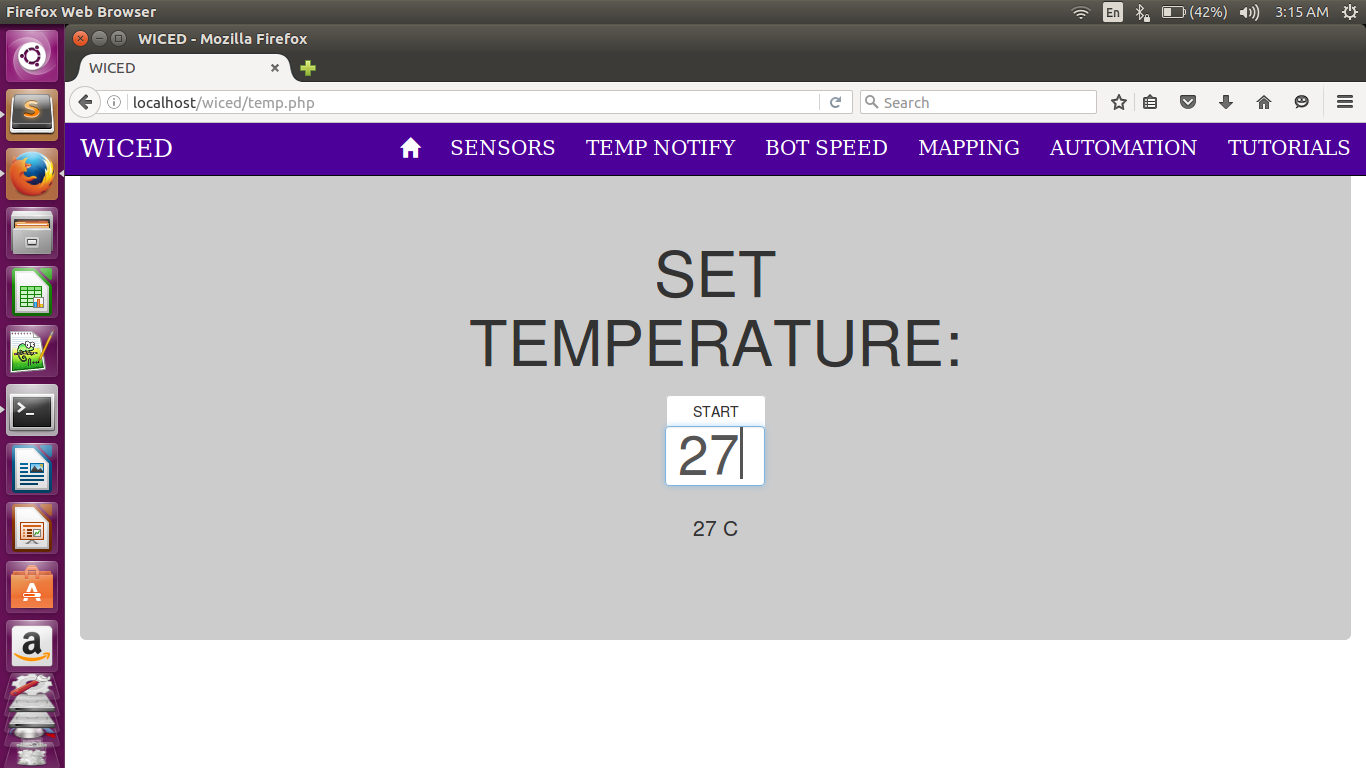
\includegraphics[scale=0.3]{temp12.png}
	\caption{Temperature Notify GUI}
	\end{figure}
	 
	 \item Selected temperature will be displayed immediately at the bottom of form.
	  \item As the atmospheric temperature exceeds above set temperature , then a popup alert will appear to notify the user.
	 
	  \begin{figure}[h]
    \centering
	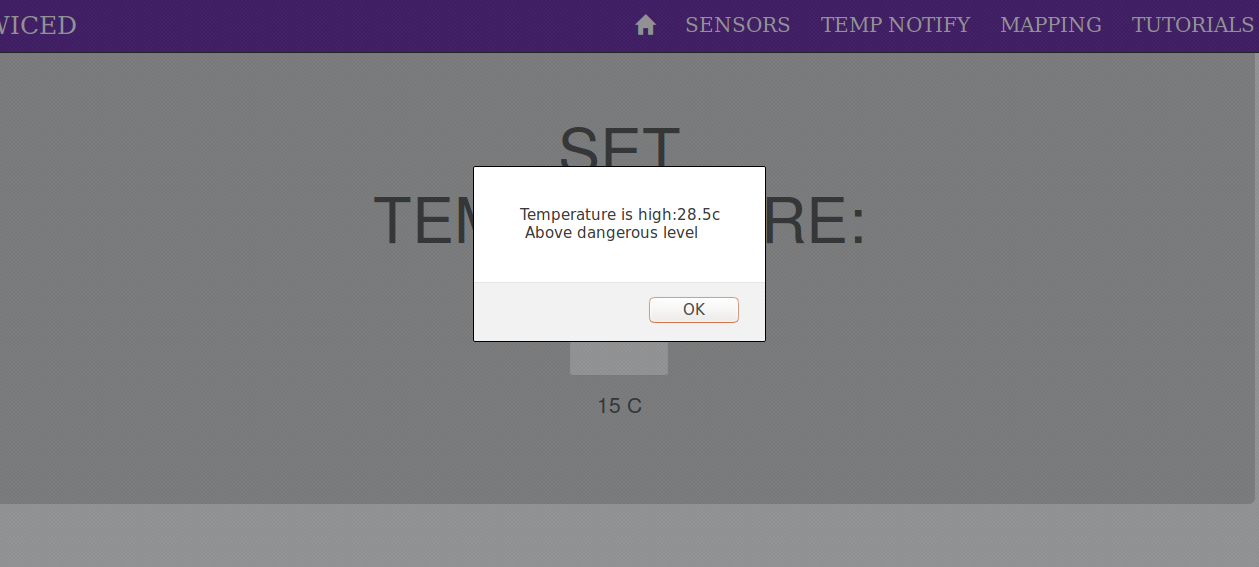
\includegraphics[scale=0.3]{popup_alert.png}
	\caption{Popup Alert}
	\end{figure}
	 \end{itemize}
	 
	 
	 \newpage
	  \subsection{How to map the path of robot ?}
	 \begin{itemize}
	 \item Open terminal and start lampp local server.
	 
	 	\begin{figure}[h]
    \centering
	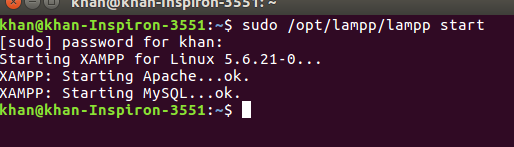
\includegraphics[scale=0.5]{lampstart.png}
	\caption{Starting Local Server}
	\end{figure}
	 
	 \item Open Open \href{https://github.com/eYSIP-2016/Wiced-Sense/blob/master/Codes/wiced_web/mapping.html}{mapping.html} page in website.
	 \item  Connect XBee using a XBee to usb adapter to a local machine.
	  
	 \begin{figure}[h]
        \centering
	    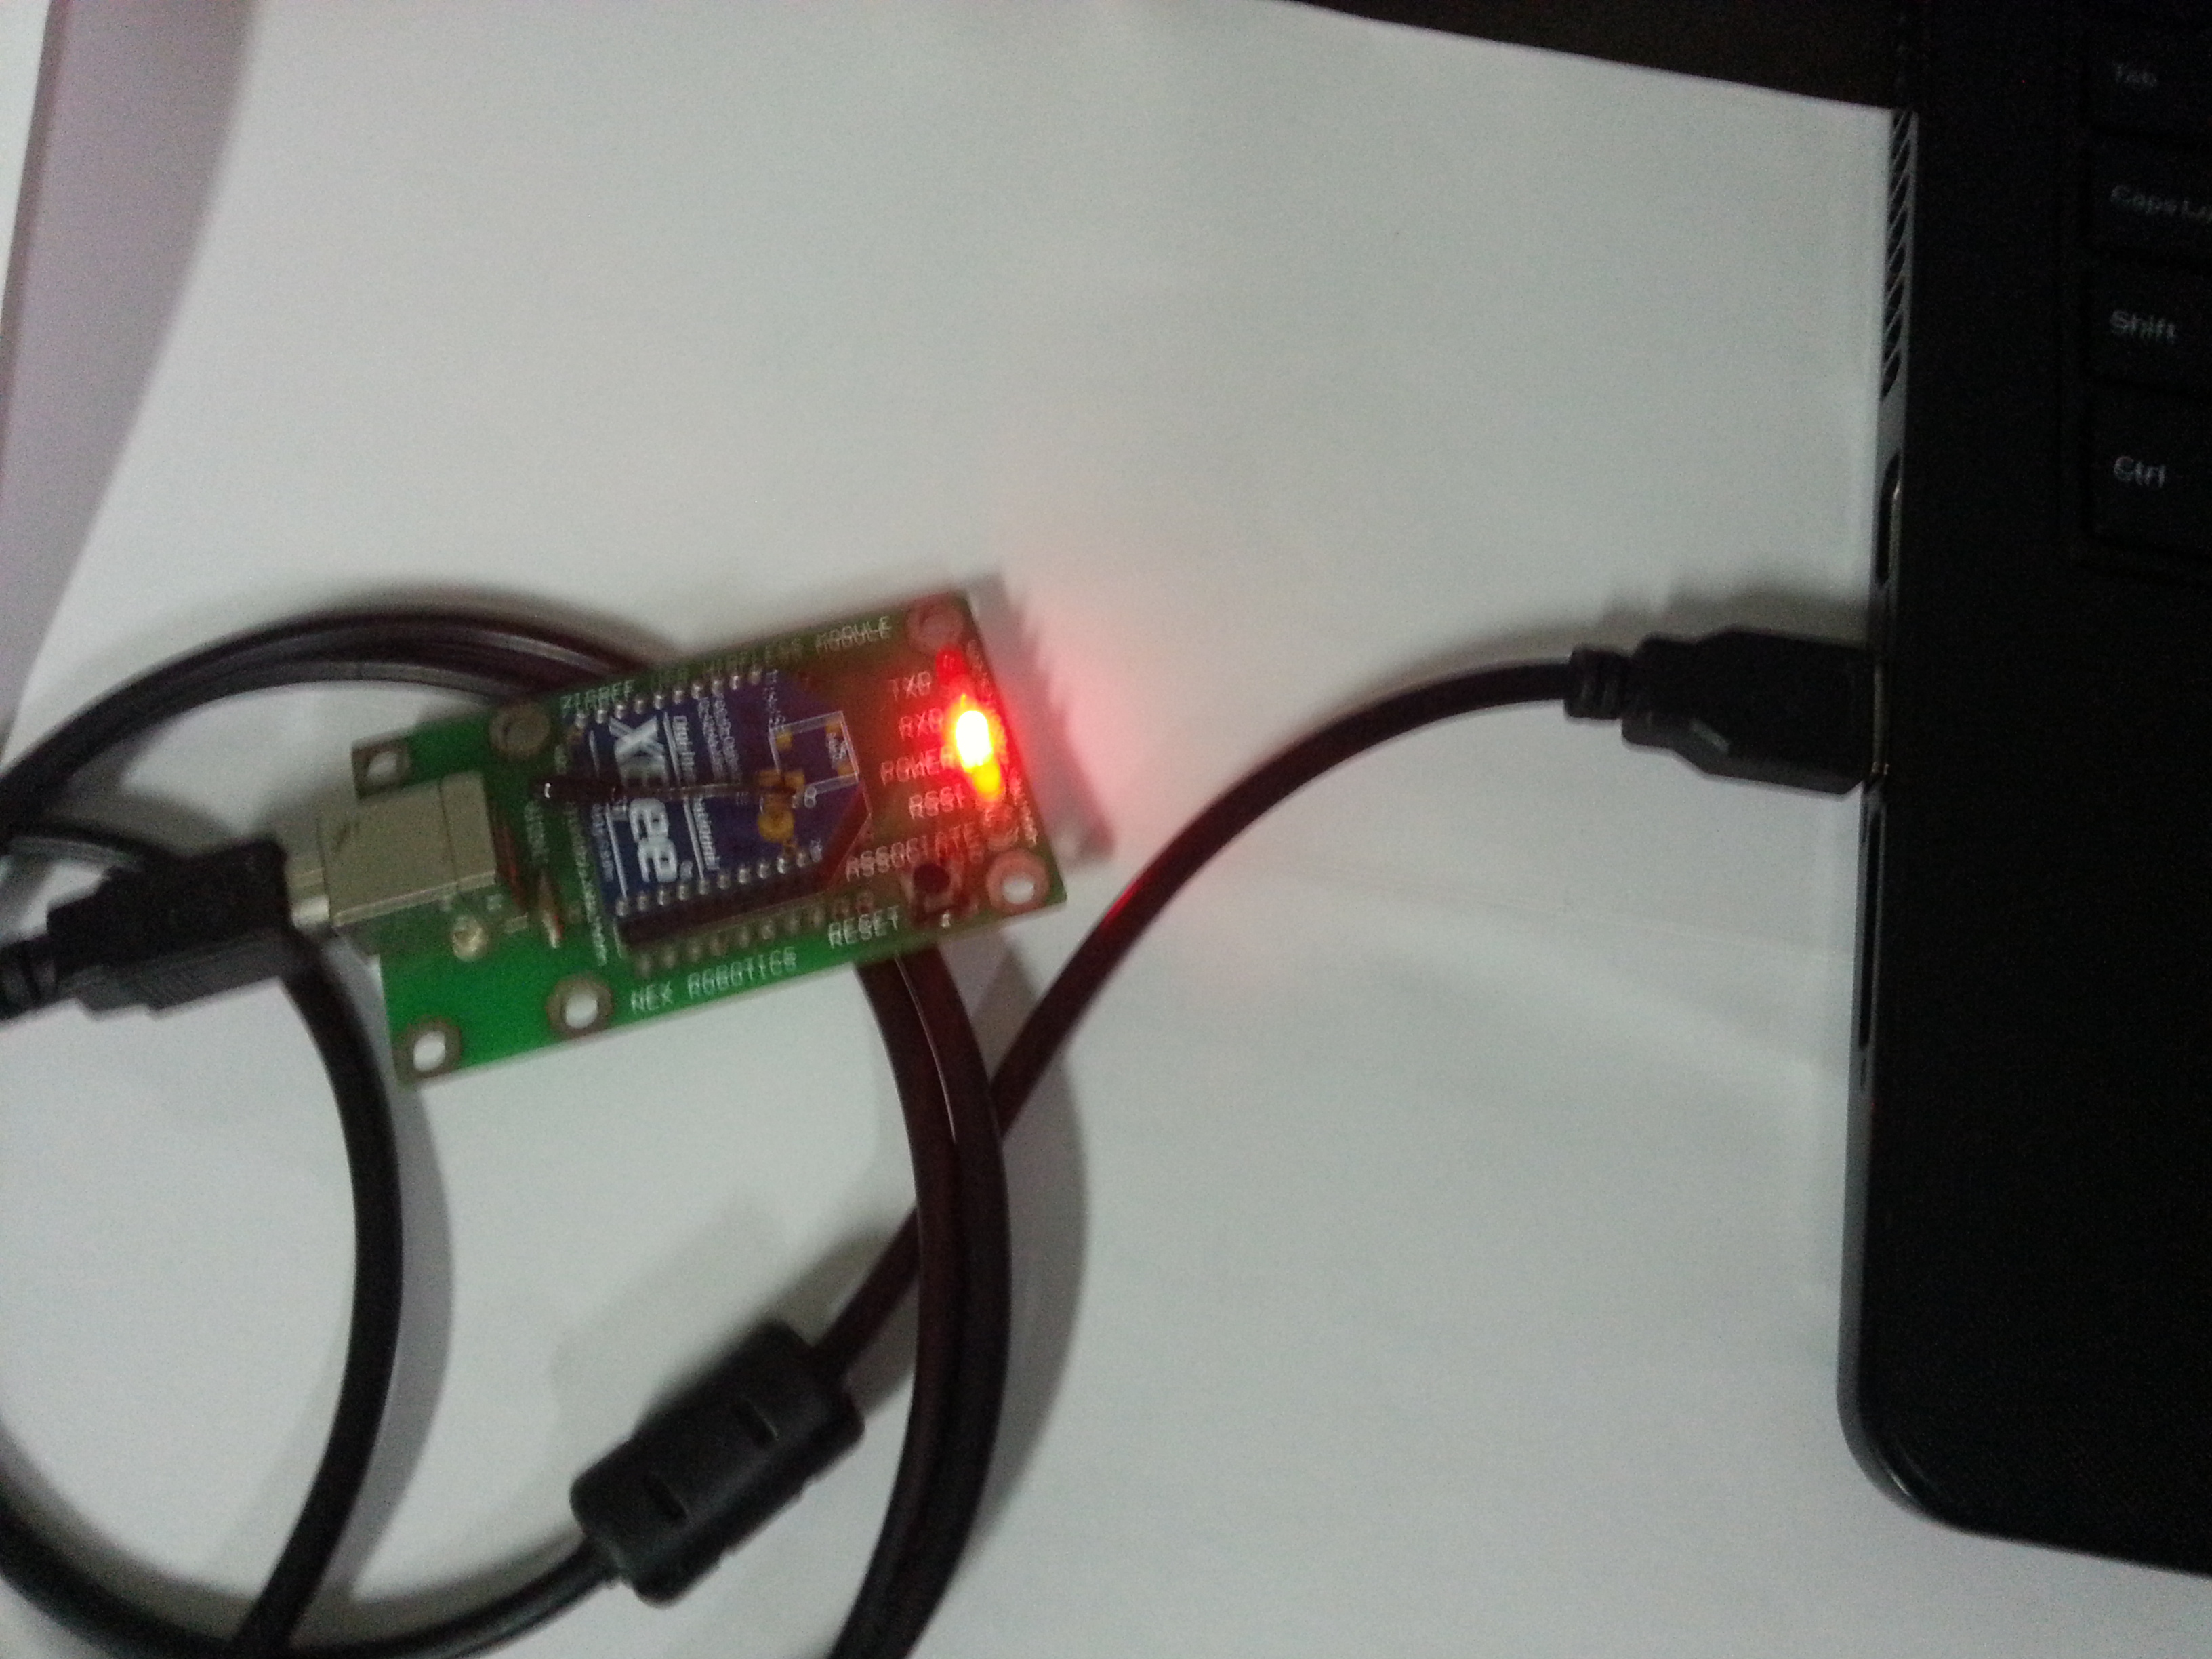
\includegraphics[scale=0.08]{20160722_194935.jpg}
	    \caption{Connecting Xbee to local machine}
	\end{figure}
	\item Place wiced sense on robot where key chain part of wiced must be facing forward .
	\begin{figure}[h]
    \centering
	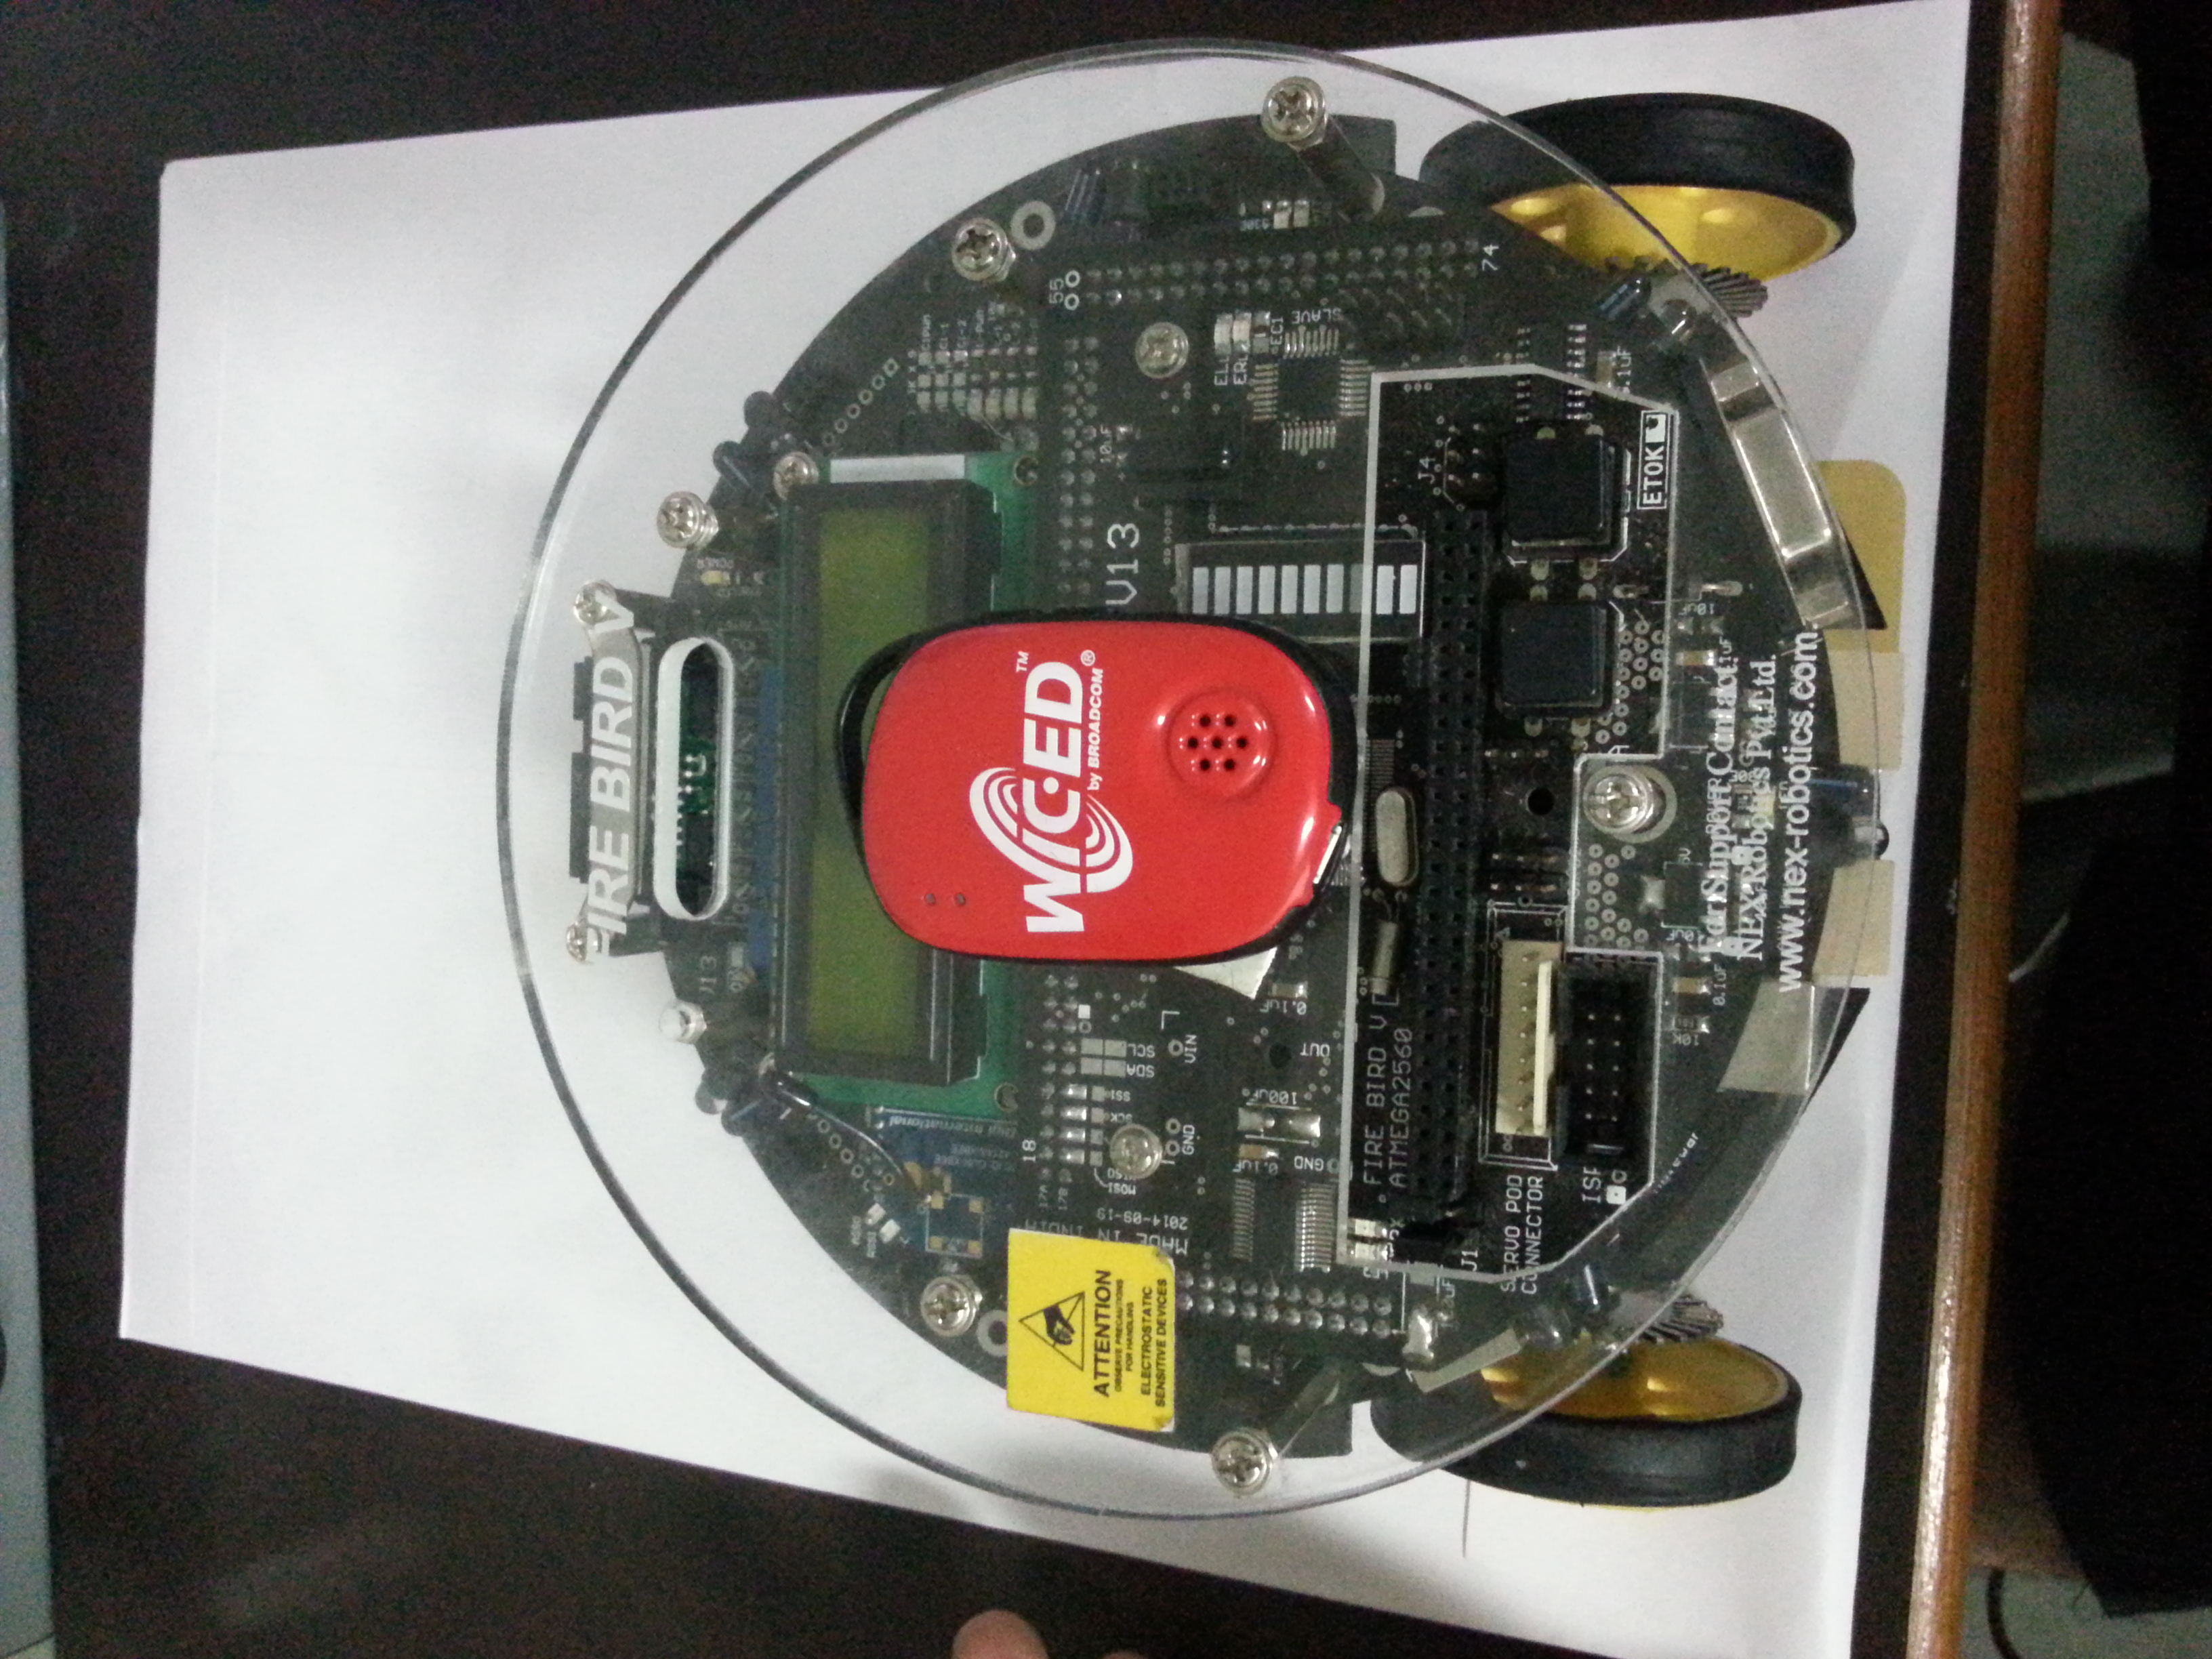
\includegraphics[scale=0.1,angle =-90]{20160722_195513.jpg}
	\caption{Mounting wiced on firebird V}
	\end{figure}
	 \item Turn ON system bluetooth and keep the bot at the start position of the path or area to be mapped.
	 
	 
	 \newpage
	\item Turn on the wiced sense by pressing the wake up button.
	 \item Do not move the robot after placing at start position.
	 \item Run wiced-sense.js file and wait for data to arrive.
	 
	 	\begin{figure}[h]
    \centering
	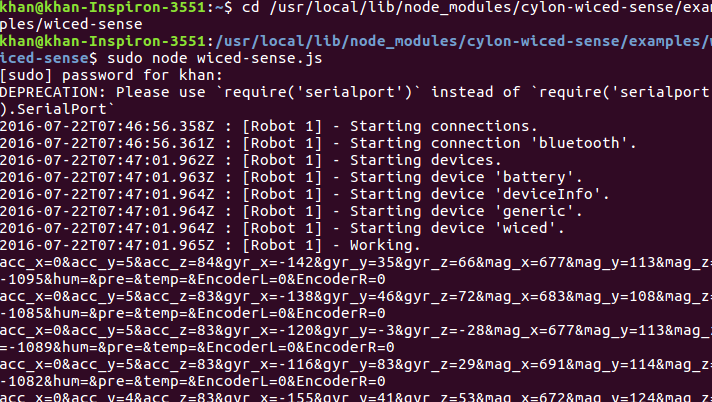
\includegraphics[scale=0.5]{data_arraives.png}
	
	\caption{Output on terminal}
	\end{figure}
	
	\item As the data arrives on terminal, immediately refresh mapping.html page.
	
		\newpage
		\begin{figure}[h]
    \centering
	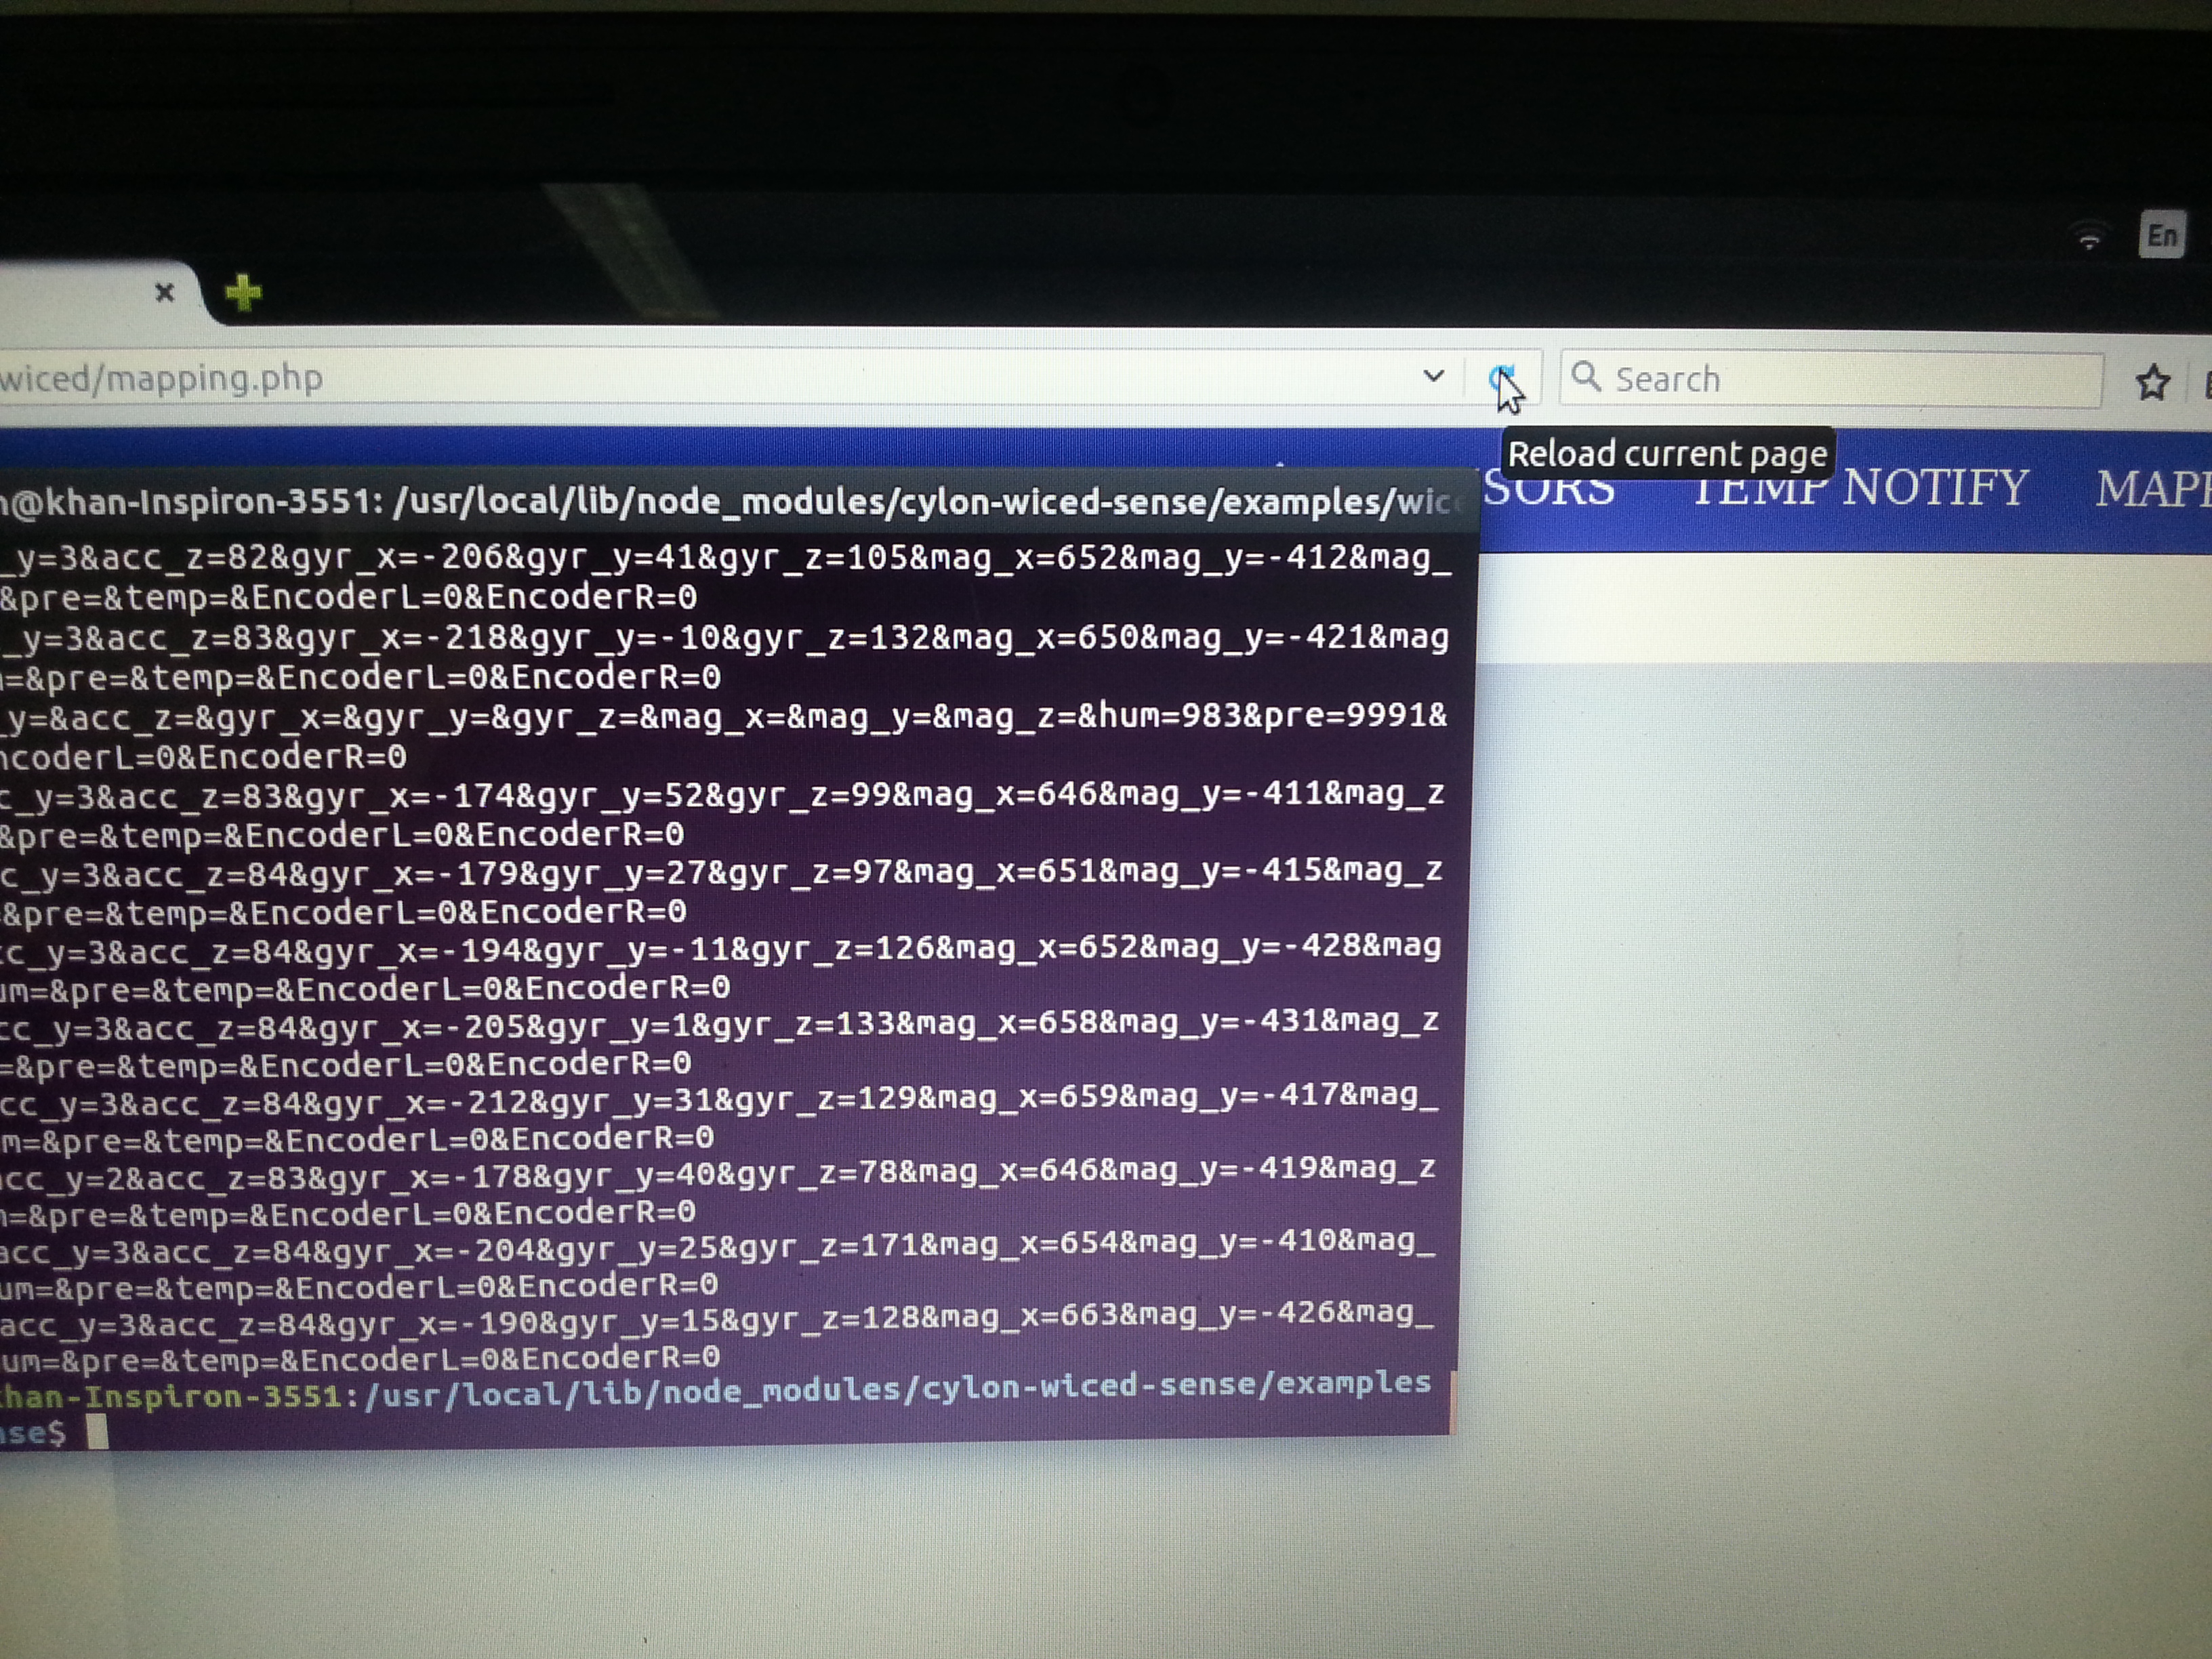
\includegraphics[scale=0.1]{20160722_195821.jpg}
	\caption{Refreshing the webpage}
	\end{figure}
	

	\item Turn on robot to move forward. As the robot moves , path is mapped accordingly in the mapping.html page.
	
	\item After mapping is done, inorder to terminate the process enter Cltr+C in terminal. Hence process will be terminated
	 	 \end{itemize}


	\end{document}